\chapter{Literature review}\label{chapter:warmup}
%Deterding et al. go on to explain that a gamified system, like a game, usually has rules and is goal oriented. Gamification is not a full-fledged game, although it utilizes many techniques that games implement such as, levels, clear goals, time constraints, badges, value conscious game design, challenge, limited resources and leader boards. It allows people to stay grounded in reality, whilestill profiting from successful game benefits like gaining access to a person’s emotions and intrinsic motivation, which in turn will help create habits. ZA ABRSTACT??
The following chapter provides an overview of the past research related to warm-up as a preparatory exercise prior to performing physical activity and conceptually related works in the domain of gamified solutions relevant to fitness and exercise. To impose structure, first the basic concepts related to warm-up and an overview of studies and results regarding the benefits of warm-up is given. Following, the concept of gamification is introduced. At the end of this chapter, a comparison between the presented approaches and our solution is made.
\section{Warm up in sports}
\subsection{Introduction}
Despite very contrasting beliefs and limited scientific evidence regarding its effectiveness in many situations, warm-up (WU) has become a standard practice among professional and
recreational athletes \cite{bishop2003warm1, bishop2003warm2, shellock1985warming}. WU in sports is defined as a period of preparatory exercise which is carried out in order to prepare the athlete for the demands of the subsequent physical activity  \cite{karvonen1992importance, woods2007warm, hedrick1992exercise}.
%karvonen skini i procitaj
Typically, WU includes a short and low-intensity preparatory activity which is followed by a stretching routine and sport specific exercise \cite{safran1989warm}. 
The purpose of WU is to enhance the subsequent competition or training performance and improve muscle dynamics to reduce the risk of sport-related injury\cite{bishop2003warm1, shellock1985warming, knudson2008warm}. 
 %HERE MENTION THE STUDIES THAT SAY THIS DOESNT HELP.  CHECK LEMON ILIEV
Nonetheless, there is still deficiency of scientific evidence on what kind of WU can influence both muscle damage prevention and performance improvement \cite{safran1989warm}.\\ %cite
\subsection{WU benefits}
Fradkin \textit{et al.} carried out a systematic review and meta-analysis of relevant studies concerning the benefits of WU on performance. They found that an adequate WU supports an improvement in performance in 79\% of the research studies analyzed. Furthermore, they pointed out that there exist little evidence supporting detrimental effects WU might have on performance and sports participants.
WU can affect the performance via variety of temperature and non-temperature related mechanisms \cite{bishop2003warm1}. 
%By performing a low intensity training routine before taking part in more demanding exercise, an increase in one's body temperature \(Magnusson 
%et al., 2000\) and muscle blood flow occurs \(Tiidus \& Shoemaker, 1995\).  
The most relevant effects of WU can be attributed to physiological mechanisms like increased muscle temperature, decreased resistance of muscle and joints (decreased stiffness), increased oxygen delivery to muscles, increased nerve-conduction rate and speeding of metabolic reactions \cite{bishop2003warm1}. 
However, the benefits of WU are not exclusively physical. Apart from the physiological changes a body undergoes during this preparatory period, it has been hypothesized that a possible psychological benefit can also be gained by following a proper WU routine \cite{bishop2003warm1,shellock1985warming}.
It has been suggested that WU can serve as a preparatory phase, providing time for athletes to concentrate and mentally prepare for the forthcoming exercise \cite{shellock1985warming}. 
%Thus, possible psychological benefits is increased mental preparedness for the forthcoming exercise\cite{bishop2003warm1}. 
For instance, in the study that investigated the link between a WU and psychological processes, Ladvig (2013) reported that athletes who performed a proper WU routine before engaging in more demanding physical activity demonstrated significantly higher levels of exercise related motivation and enjoyment. Thus, increased motivation and enjoyment is an additional psychological benefit of WU \cite{ladwig2013psychological}.
 %findings of this theisis: http://aut.researchgateway.ac.nz/bitstream/handle/10292/325/WeerapongP.pdf?sequence=1
\\*Apart from physiological and psychological benefits, WU has been suggested to have an important role in sports-related injury prevention \cite{shellock1985warming}. Unfortunately, there exist no high-quality research studies in order to draw a definite conclusion as to the effect WU has on sports-related injury prevention \cite{fields2007should}. Safran, \textit{et al.} proposed a possible bio-mechanical explanation for injury reduction with WU. The results of this study reported that warmed-up muscles in the animal models can elongate more before failure caused by increased force and length of stretch \cite{safran1989warm}. In the study of Fradkin, \textit{et al.} the current evidence regarding WU in injury prevention has been assessed. Out of five high-quality studies with sufficient data that have been systematically reviewed, three studies reported significant injury related reduction by performing WU before the physical activity, while in other two no benefits were reported. Overall, based on the weight of evidence, it has been concluded in favor of WU to decrease the risk of injury.\\
%Furthermore, Nosaka and Clarckson found that high and low intensities of WU could reduce the magnitude musculatory damage ... They proposed that 
%A search of the literature identified only one published research paper on the effects of warm-up on the severity of muscle damage (Nosaka & Clarkson, 1997).  Nosaka and Clarkson (1997) found that both high (100 repetitions of maximal concentric contraction) and low (100 repetitions of minimal concentric contraction) intensities of 
%warm-up could reduce the magnitude of mu
%scle damage as indicated by reduced 
%soreness sensation, strength and range of 
%motion loss, swelling, and creatine kinase 
%activity.  The authors proposed that warm-up 
%might help to increase muscle temperature 
%and circulation, and consequen
%tly, increase muscle and conne
%ctive tissue el
%asticity
%the majority of effects of warm up have been attributed to temperature related mechanism
\subsection{WU types}
There exist various types of WU procedures that professional and recreational athletes use as a preparatory phase for the more physically demanding exercise preparation. It is important to distinguish between WU and stretching activities. While WU mainly focuses on core body temperature elevation, stretching involves movements that stretch the muscle in order to increase the range of motions of joints or group of joints \cite{knudson2008warm}. 
Generally, WU procedures can be classified into active and passive WU procedures, and are centered on increase in core and muscle temperature. However, active and passive WU accomplish this objective through different approaches. The former involves raising muscle or core temperature by some external means (e.g. hot showers, saunas), while the latter aims to increase the body temperature through active movements of the major muscle groups (e.g. jogging, cycling, swimming) \cite{shellock1985warming, bishop2003warm2}. The most effective WU that could potentially affect the subsequent performance generally depends on the duration, intensity and the nature of the sports activity to be performed \cite{bishop2003warm2}. As each sport has its own unique requirements, it is difficult to specify a general WU routine that is beneficial and has a positive impact by maximizing the subsequent performance. Nonetheless, it is suggested that a proper WU should use general, whole-body movements and last 5-10 minutes, followed by a five minute recovery period \cite{bishop2003warm2}.  
%dodaj za fatigue
%Several studies were conducted in the 1950s-1970s to investigate the effects of warming-up on athletic performance
%(Richards, 1968). In this context, approximately 60% of these studies found that warm-up was better
%to perform than no warm-up, whereas ~11% found that no warm-up was better, and the remaining ~29% found
%no significant differences between different protocols of warm-up and no warm-up (Blank, 1955). 
%tu sad das ove linkove
%(Generally, a warm-up to minimize impairments and enhance performance should be composed of a submaximal intensity aerobic activity followed by large amplitude dynamic stretching and then completed with sport-specific dynamic activities.
%these say that some stretching is ok
%http://www.jospt.org/doi/pdf/10.2519/jospt.1994.19.1.12
%https://www.ncbi.nlm.nih.gov/pubmed/21373870
%The efficacy, and characteristics, of warm-up and re-warm-up practices in soccer players: a systematic review. This review demonstrated that a static stretching WU reduced acute subsequent performance, while WU activities that include dynamic stretching, PAP-based exercises, and the FIFA 11+ can elicit positive effects in soccer players. The efficacy of an active RWU during half-time is also justified.
%ovo se placa nesto 
 %http://greatist.com/fitness/stretching-dynamic-warmup-040413
\\*Although considering the aforementioned benefits and the fact it is widely recommended to undertake the practice of WU, many amateur and recreational athletes do not seem to perform a proper WU before an exercise \cite{fradkin2010effects}. The reasons for this are manifold. Some people do not realize the importance of WU, find it tiresome or being pressed for time and eager for instantaneous results, start with the more strenuous activity immediately. A recent survey carried out by Fradkin, \textit{et al.} which included 1040 golfers and their WU habits, revealed the most common reasons for not warming-up. The survey showed that out of all the questioned golfers, over 70\% never or rarely warm-up. The most common reasons for not performing a proper WU routine were the perception that WU is needless (38.7\%), lack of time (36.4\%) and that they do not want to be bothered with this routine (33.7\%).
% A survey of 1040 randomly selected golfers was conducted over a 3-week period in July 1999. Information about golf participation, usual warm-up habits and reasons for these warm-up behaviours was obtained by a verbally administered self-report survey. Over 70% of the surveyed golfers stated that they never or seldom warm-up, with only 3.8% reporting warming-up on every occasion. The most common reasons why golfers warmed-up included to play better (74.5%), to prevent injury (27.0%), and because everyone else does (13.2%). Common reasons for not warming-up were the perception that they don't need to (38.7%), don't have enough time (36.4%) and can't be bothered (33.7%).
These results suggest that educational and motivational solutions with primary focus on the benefits of WU, including injury prevention, need to be developed and implemented in order to increase the proportion of athletes who engage in WU routines before every strenuous exercise. One possible solution is the usage of \textit{Gamification} in motivating athletes to perform WU more regularly. 
\pagebreak
\section{Gamification}
Having outlined the basic concepts regarding Warm-up procedures, the following section sheds light 
on the dimensions of Gamification. In order to tie in with the idea of comparing both concepts, after  introducing Gamification in further detail, the emphasis will be placed upon taking a look at the 
gamified solutions in the domain of fitness and health. 
\subsection{Introduction}
%http://link.springer.com/chapter/10.1007%2F978-3-319-07127-5_23
%(http://www.enterprise-gamification.com/mediawiki/index.php?title=Category:Gamification_Design_Elements)
% are commonly used 
%check this here https://badgeville.com/wiki/health
%% add gamification example reference
% http://www.enterprise-gamification.com/mediawiki/index.php?title=Gamification_Examples
In recent years, there has been a tremendous increase in popularity of video games inspired software solutions designed to address issues in a variety of functional areas, incentivize consumer behavior or increase motivation and the desire for achievement. What these software solutions all have in common is that they are based on the concept of \textit{Gamification}. This term has begun to rise in popularity in 2010 (Figure \ref{fig:buzz}), and since then has been a trending topic. %ovde dodaj 
%It has proved to be an effective tool for certain businesses for developing new skills, solve problems, improve results or address.
\begin{figure}[h]
    \centering
    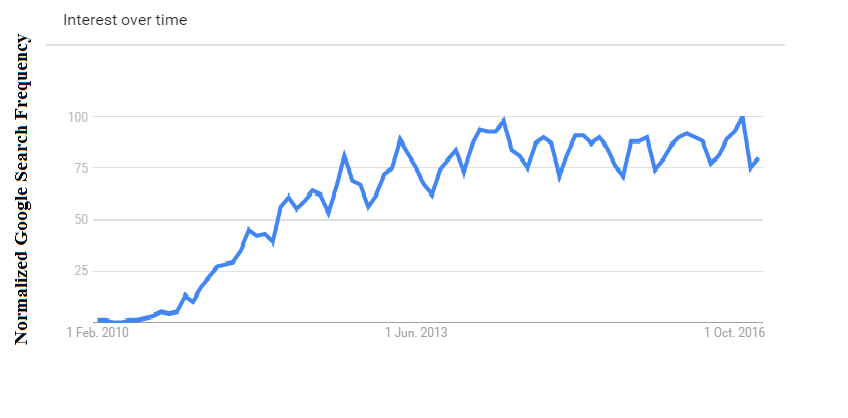
\includegraphics[width=\textwidth]{buzz}
    \caption{Google search frequency of the term \textit{gamification} from Janauary 2010 through January 2017. Data source: Google Trends, www.google.com/trends}
    \label{fig:buzz}
\end{figure}
Gamification is being used and studied in various domains, from education and academic performance to health care, finance, company culture building and recruitment, to name a few \cite{gamificationExamples, gamificationWiki, enterpriseGamify}. Large companies like Nike \cite{nikePlus}, Deloitte \cite{deloitte}, Starbucks \cite{starbucks}, Coca Cola \cite{coke} and Toyota \cite{toyota} have all used gamified solutions in order to increase customer loyalty, change behaviors, 
and drive innovation. %example u STUFF
Moreover, there is an increasing number of startups (e.g. Foursquare, CodeAcademy) that have gamification  at  their  core \cite{codeacademy} or offer assistance to enterprises to gamify their existing services (e.g. Badgeville \cite{badgeville}). Hamari \textit{et al.} reported on an increasing popularity of gamification related researches in the academia \cite{hamari2014does}. Figure \ref{fig:pub} gives an overview of the increase of writing on this topic. The figure includes only the number of publications for every year for the term \textit{Gamification} and excludes patents and citations. 
\begin{figure}[h]
    \centering
    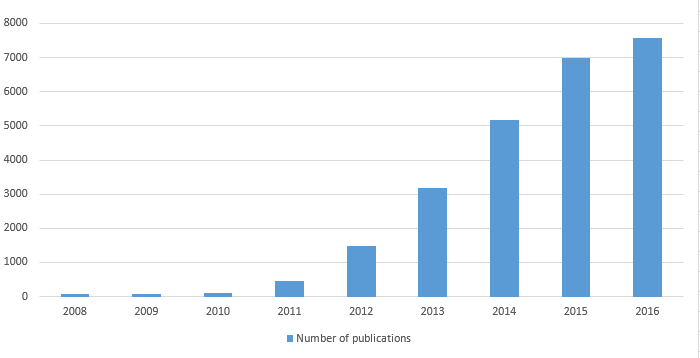
\includegraphics[width=\textwidth]{pub}
    \caption{Search hits on 'Gamification'. Data source: www.scholar.google.com}
    \label{fig:pub}
\end{figure}
It is worth noticing that the appearance of the term Gamification titles of publication has been increasing more rapidly than search hits for the same term (see Figure \ref{fig:buzz}). This suggests that Gamification is becoming more popular in academic circles as a research topic. 
\section{Theories of Motivation}
The player forms the root of Gamification and, in any system, the outcome is affected and driven by his motivation (Zichermann \& Cunningham, 2011, p. 15). Therefore, to understand the potentials and fundamental aspects behind Gamification, one important part is to understand what drives people's motivation. Thus, psychology is  essential  to  Gamification  in order to understand  how  human  nature  works  and  how  it can  be  influenced  in  order  to  create  an  effective  Gamified  system. For this reason, the next sections introduce different views from psychology about motivation and explain what has to be considered in terms of truly engaging individuals. There are two main purposes of this section. The first is to provide a suitable overview of the subject itself and to introduce terms that will be used later in the discussion. The second purpose is to present theories that describe and explain various psychological effects that games have on players and how can they be used to enhance user's engagement and motivation when interacting with a gamified system. Two important theories that are regarded as important foundations for  the  concept of Gamification are presented. First, the Self Determination theory introduced by Ryan and Deci, and then the State of Flow by Mihaly Csikszentmihalyi are discussed. 

\subsection{The Rules of Motivation}
Gamification is about motivating  individuals to act in a certain way, or at least develop an inclination for specific behavior,  whether  it's  visiting  the gamified  system  more  often,  learning a new language, or exercising more. 
The word \textit{motivation} originates from Latin \textit{motivus} and stands for ``serve to move''. In other words, motivation can be interpreted as \textit{to be moved to do something}. It can be defined as ``those forces within an individual that push or propel him to satisfy basic needs or wants'' \cite{pardee1990motivation}. One of the most influential researchers in the domain of human motivation and behavior, Richard M. Ryan \& Edward L. Deci (2010b), argue that people \textit{can be moved} to act by various types of factors, as so with highly diverse experiences and consequences. For example, people can be motivated because they value the activity they perform, or because there exists some external influence and pressure. Furthermore, they point out that each person has different amounts and also different kinds of motivation. That is, each person is different in level (i.e. how much motivation) and orientation (i.e. what type of motivation) of their motivation, whereas orientation might be a goal which gives rise to action and therefore governs human behavior. \\*

\subsection{Self Determination Theory}
%deci ima dva papera
An aspect to understanding player motivations is by questioning the source of one's motivation. One of the most influential motivational theories is the Self Determination Theory (SDT) introduced by Ryan \& Deci. It is an empirically derived theory of human motivation that makes distinctions between different types of motivation in terms of reasons and goals that cause the respective action. That is, SDT proposes that behaviors that are intentional might vary in the extent to which they are \textit{self-determined} versus \textit{controlled}. This means that behaviors can vary in the extent they are experienced as being freely chosen and coming from one's self in contrary to being pressured or controlled externally. When these behaviors are experienced as freely chosen they are considered self-determined or autonomous, whereas the extent they are experienced as coerced, they are considered controlled \cite{deci1994promoting}. Having this in mind, SDT distinguishes between \textit{Intrinsic} and \textit{Extrinsic} motivation. The first type of motivation, as the word \textit{intrinsic} already suggests, refers to performing an activity for the inherent satisfaction. When intrinsically motivated, a person is moved to act because the activity is challenging, interesting and enjoyable on its own rather than because of some external prods, pressures, or rewards. On the other hand, extrinsic motivation refers to performing an action because it leads to \textit{separable outcome}. That is, there is some external reward or influence which drives the person to accomplish the task (Deci  \& Ryan, 2000). The comparison between people intrinsically and those extrinsically motivated reveals that the former have more interest, excitement, and confidence which in turn, can not only enhance performance, persistence, and creativity but consequently boost vitality, increase self-esteem and general well-being \cite{ryan2000self}. Though this division is for most people intuitively understandable, it is not always as clear as it may seem. For example, as the SDT theory states, \textit{motivations are fluid}. Hence, people can convert extrinsic motivators to intrinsic if they internalize the desire to do so. To put it more simply, in a situation where the extrinsic motivator is found meaningful, pleasurable and consistent with a person's worldview, it can be perceived and adopted as if it was intrinsic \cite{zichermann2012}.
Although, in one sense, intrinsic motivation can exist within an individual, in another sense, it can exist in the relation between the individual and the activity one performs. Having that in mind, it is important to point out that not everyone is intrinsically motivated for the same activities and that not everyone is intrinsically motivated for any particular activity \cite{ryan2000intrinsic}. In SDT, the \textit{basic psychological need satisfaction} is assumed to be the core motivational mechanism that directs human's behavior. SDT postulates three innate psychological needs (see Figure \ref{fig:ss} ), that are ``essential for ongoing psychological growth, integrity, and well-being'' and all three of them play a necessary part in optimal development, hence none can be disregarded without significant negative consequences. These needs are the need for autonomy, competence and relatedness and when individuals experience them, they become self-determined and intrinsically motivated to pursue thing that interest them \cite{deci2000and}. %https://selfdeterminationtheory.org/SDT/documents/2010_VandenBroeckVansteenkisteNSscale_JOOP.pdf
\begin{itemize}
\item \textbf{Autonomy} represents individuals' innate desire to feel \textit{free} and to experience a sense of choice and psychological freedom when carrying out certain activities \cite{deci2000and}. Situations in which individuals are provided with the opportunity to choose freely, accompanied with a positive feedback, have been shown to influence and improve autonomy and, hence, the intrinsic motivation of individuals [ryan 2006]. For example, students  are  autonomous when they willingly spend time and energy for completing their assignments. 
\item \textbf{Competence} represents individuals' innate desire to feel effective when interacting with the environment. For example, students are competent in cases when they feel they can meet the challenges of their schoolwork. Furthermore, Deci \& Ryan (2000) point out that positive feedback can signify effectance and provide a satisfaction of the need for competence, thus enhancing intrinsic motivation, whereas negative feedback that convey ineffectance, tend  to
diminish the sense of competence and hence undermine intrinsic motivation. 

%A. P. Hill, "A Brief Guide to Self-Determination Theory," September 2011. [Online]. Available: http://www.heacademy.ac.uk/assets/hlst/documents/projects/round_11/r11_hill_guide.pdf. [Accessed 10 April 2013].

\item \textbf{Relatedness} corresponds to experiencing meaningful connection to others, that is, to be a member of a group, to love and care and to be loved and cared for \cite{broeck2010capturing}. This psychological need is satisfied when individuals experience a sense of togetherness and develop a close and intimate relationship with others. \\*
\end{itemize}
\begin{figure}[h]
    \centering
    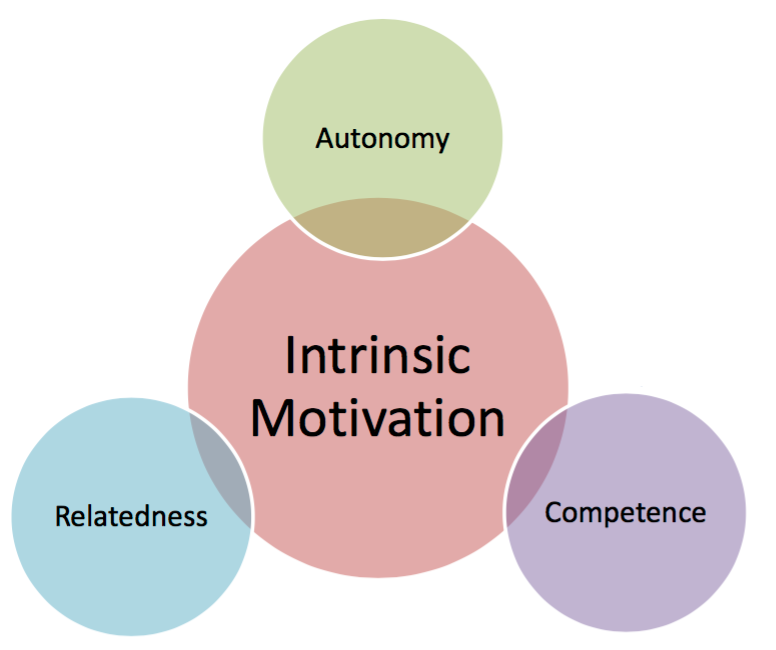
\includegraphics[width=0.6\textwidth]{ss}
    \caption{Basic psychological needs according to Ryan, R.M. \& Deci E.L.}
    \label{fig:ss}
\end{figure}
The specification of autonomy, competence, and relatedness is important because it allows the prediction of variables that can affect individual's intrinsic motivation and the development of their extrinsic motivation \cite{deci1994promoting}. These needs can be achieved by means of diverse game elements, which will be discussed in detail in the next section.\\*\\*
Despite the observable evidence that humans, in general, can have intrinsic motivational tendencies towards some activities, this bias appears to manifest only in certain conditions and circumstances. Hence, SDT also places much emphasis on understanding conditions that enhance and sustain versus subdue and diminish intrinsic motivation.  A sub-theory of SDT called Cognitive Evaluation Theory (CET) was presented by Deci and Ryan (1985) and focuses on social and environmental factors that promote or undermine this type of motivation using language that reflects the assumption that intrinsic motivation, as an inherent bias, is rather catalyzed than caused when individuals are in appropriate socio-enviromental circumstances (Ryan  and  Deci  2000;  Ryan and Deci 2000b). In other words, intrinsic motivation does not occur by itself, but represents the outcome of one's interaction with the environment and one's interests and preferences. That is, intrinsic motivation ``will flourish if circumstances permit'' \cite{ryan2000self}. Furthermore, CET, which focuses mainly on the fundamental needs for competence and autonomy, argues that interpersonal events and structures, such as rewards, communication or feedback can increase intrinsic motivation for certain actions because they satisfy the basic psychological need for competence. Accordingly, it is predicted that optimal challenges, positive feedback and freedom from degrading evaluations promote intrinsic motivation, while tangible rewards, threats,  deadlines  and  directives decrease it (Ryan \& Deci, 2000). Furthermore, CET also argues that the satisfaction of the psychological needs for competence will not enhance intrinsic motivation unless they are joined by a sense of autonomy. Hence, people must perceive that their behavior is self-determined in order for intrinsic motivation to be maintained or enhanced. In other words, for a high level of intrinsic motivation, the needs for competence and autonomy must both be satisfied (Ryan \& Deci, 2000). It is important to point out, as stated by Ryan \& Deci, that people will be intrinsically motivated for certain activities only when they are intrinsically captivating for an individual, that means activities that offer a degree of novelty, challenge or aesthetic value. Activities that do not provide such appeal, will not be experienced as intrinsically motivated. \\*\\*
Even though intrinsic motivation is of great importance, most of the activities people engage in are not intrinsically motivated. Such activities, being uninteresting and unsatisfactory for individuals  require external \textit{push} in order to be realized. This motivation, contrary to intrinsic motivation which refers to doing an activity simply for the enjoyment of the activity itself, is known as extrinsic motivation. It refers to performing certain activities because it is expected to result in some additional outcome or reward that have an instrumental value for the individual performing that action \cite{ryan2000self}. In general, extrinsically motivated behaviors are ones that would not happen instinctively, and hence must be prompted by an intrumentality \cite{deci1994promoting}. Various studies demonstrated that in specific circumstances extrinsic motivation can sustain intrinsic motivation, thus suggesting that extrinsically motivated behaviors can also be self-determined \cite{deci1994promoting}. Extrinsically motivated behaviors become self-determined through the process of \textit{internalization} and \textit{integration}. Internalization involves transforming internal regulatory processes into internal regulatory processes, while integration corresponds to the process of integrating these now internalized values and regulation into one's self \cite{deci1994promoting}. There exist four types of extrinsic regulation that can result from different types of internalization and integration, which were introduced within SDT as a subtheory called Organismic Integration Theory (OIT) \cite{ryan2000intrinsic, ryan2000self, deci1994promoting}. For instance, students who work on their assignments because they personally understand its importance for their future career and those who do it only to adhere to their parents' control are both extrinsically motivated. Even though both cases involve instrumentalities rather than enjoyment, the former entails personal endorsement and a feeling of choice while the latter associates only with an external regulation.\\*\\*
Figure \ref{fig:tax} illustrates the IOT taxonomy of motivational types arranged from left to right in terms of the degree to which the motivation originates from the self (i.e. are self-determined).
\begin{figure}[h]
    \centering
    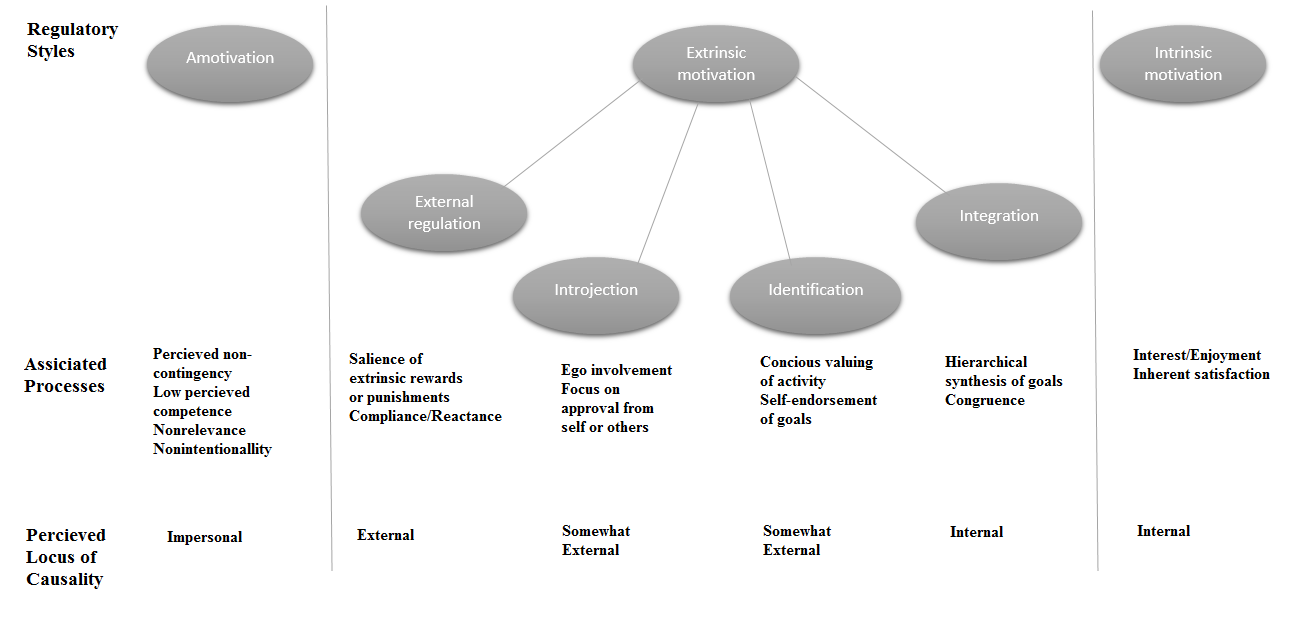
\includegraphics[width=\textwidth]{taxm}
    \caption{Based on Ryan, R.M. \& Deci E.L.(2000). Self-Determination Continuum showing types of Motivation}
    \label{fig:tax}
\end{figure}
First, extrinsically motivated behavior that is the least autonomous is known as \textit{External Regulation} and is regulated through some external means, such as rewards and constraints. For example, an athlete who participates in the Olympics only to obtain a medal represents an instance of externally regulated behavior. In case of \textit{Introjected regulation}, individuals begin to internalize the reasons for their action. However, this internalization only replaces the external source of motivation with an internal one, such as guilt, worry or shame. That is, when people are motivated to perform activity in order to maintain feeling of worth. An example for introjection is the athlete who goes to the practice just because he would feel guilty if it has been skipped. A more autonomous type of extrinsic motivation, \textit{identification}, manifests when a person identifies with the importance of some behavior and accepts it as a personal regulation only because it benefits the athlete in achieving a specific goal. An example for this behavior is a runner who does not like weight lifting, but nevertheless chooses to to do it because it will positively impact her future performance. \textit{Integrated regulation}, as the most autonomous of extrinsic motivation that shares many qualities with intrinsic motivation, is a form of motivation that arises when an individual has fully assimilated the identified regulation within himself. An example of integrated regulation is an athlete who chooses to postpone the night out with his friend in order to be in good shape for the next day's tournament. Integration together with intrinsic motivation represent the core for self-determined functioning and they both share the qualities that constitute self-determination. Even though they might seem quite similar, they are different in the sense that intrinsically motivated behaviors are ``autotelic in nature'' while, on the other hand, integrated behaviors are ``instrumentally (though freely) performed'' for the outcome that is self satisfactory.  Finally, the self-determination continuum is closed with  \textit{amotivation} which represents ``non-regulation'' from the SDT perspective as it refers to a state where intentions to act are non existent. A person amotivated towards exercise would not exercise at all, 
or engage in exercise in a passive and disorganised  manner \cite{vallerand2007intrinsic, ryan2000intrinsic, deci1994promoting}.

\subsubsection{Gamification and SDT}
In their book \textit{For the win. How Game Thinking can revolutionize your business}  Werbach and Hunter state that ``games are perfect illustration of the lessons of SDT''. They point out how even simple games activate intrinsic needs for autonomy (because it is up to the player how to solve a challenge), competence (sense of accomplishment if certain goal is achieved) and, lastly, relatedness (when the the achieved results are shared among group of friends). The same way as games, Gamification uses these three innate motivators in order to generate results.
What are the specific takeaways for a successful gamification?
- Rewards can crowd out fun
- Boring can be engaging
- Tune your feedback
Tangible and expected extrinsic rewards can damage intrinsic motivation and interesting tasks (Werbach and Hunter,2012, p.60). On the other hand, extrinsic rewards can also have a positive effect when people need to accomplish boring
tasks (Werbach and Hunter,2012, p.62).
NOT COMPLETED-TODO
\\*

\subsection{State of Flow}

Mih\'{a}ly Cs\'{i}kszentmih\'{a}lyi, one of the most recognized game psychologists and a professor at University of Chicago, described in 1975 for the first time the phenomenon of \textit{flow}. Being fascinated by artists who would essentially get lost in their work Cs\'{i}kszentmih\'{a}lyi argued how, creative people might differ from one another in many ways but they always have one thing in common. They love what they do. Their love for a particular activity is not because of a potential outcome or a reward. What drives them is solely the opportunity to do what they enjoy doing \cite{csikszentmihalyi1996flow}. Athletes often refer to this concept as ``being in the zone,'' religious mystics
as being in ``ecstasy,'' artists and musicians as ``aesthetic rapture'' \cite{csikszentmihalyi1997finding}. In order to explain this experience, Cs\'{i}kszentmih\'{a}lyi has interviewed individuals willing to devote many hours to their avocations without asking for external rewards. After a series of studies, based on the individuals' responses regarding their emotions while performing certain activity they enjoy, Cs\'{i}kszentmih\'{a}lyi  developed a theory of optimal experience based on the concept of \textit{flow}, which he describes as 
``the state in which people are so involved in an activity that nothing else seems to matter; the experience itself is so enjoyable that people will do it even at greater cost, for the sheer sake of doing it'' \cite{flow1990psychology}. Flow is also considered as an optimal state of intrinsic motivation, where people become absolutely immersed in what they are doing, they forget about physical feelings, passage of time, and their ego fades away \cite{lithiumGamification}. 
It represents a state in which one feels in control, fully immersed and motivated, at the top of its abilities and neither overwhelmed by difficulty nor uninterested. Cs\'{i}kszentmih\'{a}lyi \textit{et. al} (2004) state the flow experiences are relatively rare in everyday life, however, various activities are able to produce them, provided certain conditions are met. They further argue that three conditions have to be met in order to achieve a flow state. First, a state of flow needs clearly defined set of goals which must guide the user and give purpose to the behavior \cite{csikszentmihalyi2014flow}. However, sometimes the goals of some activities cannot be perfectly clear for the individual, as in the case of creative activities. Nonetheless, it is possible for a person to develop a strong personal sense of what is intended to be done by performing the activity \cite{kiili2006evaluations}. The second condition for obtaining the state of flow is the presence  of clear and immediate feedback. It informs the user if he/she is succeeding in a specific goal and how to adjust his or her performance according to the ``continually  changing environment demands'' \cite{csikszentmihalyi2014flow}. Lastly, one of the most important condition is to maintain balance between perceived challenges and perceived skills \cite{csikszentmihalyi2014flow}. When experiencing a flow, a person's skill is at just the right level to cope with the situational demands.\\*
Nakamura and Cs\'{i}kszentmih\'{a}lyi (2012) further argue that under these three conditions, individuals can enter a state with the following characteristics:
\begin{itemize}
\item Control. A sense that one has skills sufficient enough to minimize the margin of error to close to zero and, therefore, can in principle deal with and fully enjoy the current situation because one knows how to respond to any anything that can happen next \cite{csikszentmihalyi2014flow}. Moreover, this sense of control is believed to be one of the important flow antecedents in games\cite{kiili2006evaluations}. 
\item Action–awareness merging. The flow state is so involving that, during it, it affects the individual in a way that the activity performed becomes spontaneous and automatic.
\item Concentration. While in flow, one experiences intense and focused concentration on what is being done in the present moment. By doing so, one is able to forget all unpleasant things beyond the performed activity since the person is left with no cognitive resources for irrelevant information processing \cite{kiili2006evaluations}. 
\item Loss of self-consciousness. During flow, the self disappears from one's awareness. That is, while thoroughly engrossed with an activity, as in the state of control, few cognitive resources are
available for self-scrutiny \cite{kiili2006evaluations}.
\item Distortion of temporal experience. Typically, the sense of time
during the flow experience tends to bear little relation to the actual passage of time, a
sense that time has passed faster than normal.
\item Autotelic experience. Autotelic experience refers to an activity that is performed simply because it is intrinsically rewarding and not with the expectation of some future benefit.
\end{itemize}
Whenever individuals try to reflect on their flow experiences, they tend to mention some and often all of these characteristics. The described conditions and characteristics of flow are known as the \textit{nine dimensions of the state of flow}, where the first five dimensions can be considered flow antecedents and the rest indicators of flow experience  \cite{kiili2006evaluations}.
According to Cs\'{i}kszentmih\'{a}lyi, flow often tends to occur in situations when we face challenges that match our skills and abilities. That is, it occurs when we perform tasks and activities that are neither too difficult nor too easy with respect to the set of skills we possess - a balance of the relationship between challenge and ability \cite{csikszentmihalyi1997finding, flow1990psychology, csikszentmihalyi1996flow}. This balance is referred to as \textit{flow zone}. When the task is too difficult (i.e., the skill cannot meet the challenge), that is when one is above the flow channel, we are likely to experience anxiety. In the opposite case, when the task is slightly too easy and task challenges do not come close to our ability, the result is boredom. Furthermore, if a person's skills improve over time, the challenge difficulty also needs to increase along with the improved skill-set. Figure \ref{fig:flowZone} depicts the graphical representation of the state of flow, where y-axis represents the difficulty of the challenge and the x-axis skill set required to meet the specific challenge. Moreover, diagram contains the flow-channel, as well as the anxiety-region and the boredom region. 
\begin{figure}[h]
    \centering
    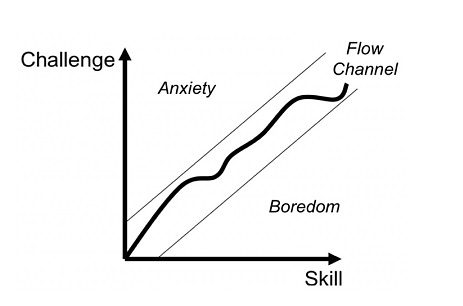
\includegraphics[width=0.6\textwidth]{flowZone}
    \caption{Based on the original model of the flow state)}
    \label{fig:flowZone}
\end{figure}
Over the years, new theories regarding the state of flow have been introduce and the concept flow was redefined by introducing eight experimental channels rather than previously mentioned quadrants \cite{nakamura2014concept}. Figure \ref{fig:flowModel} shows the refined challenge/skill space which now contains a series of concentric rings, associated with increasing intensity of experience.
\begin{figure}[h]
    \centering
    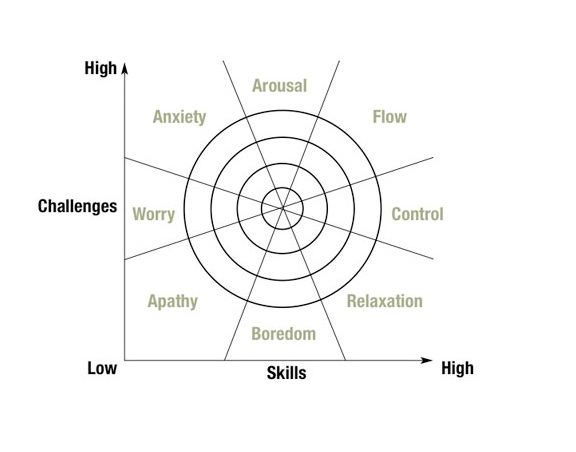
\includegraphics[width=0.6\textwidth]{flow-model}
    \caption{The current model of the flow state \cite{nakamura2014concept}}
    \label{fig:flowModel}
\end{figure}
Based on the current model of the flow state \ref{fig:flowModel}, the flow is experienced in situation when challenges and
skills are above the individual's average levels. When the task is slightly too easy (or slightly too hard) we fall out of the state of flow and enter a state where we feel in control (or the state where we feel aroused if the task is slightly too hard). When the difficulty of the task performed way above our skills, we are tend to experience anxiety. On the other hand, if challenges do not come close to our ability, we will tend to experience boredom. In cases they are below, apathy is experienced. The new model also deals with the intensity of the experience and states the it increases with distance from the individual's average levels of challenge and skill, as shown by the concentric rings \cite{nakamura2014concept}.
Cs\'{i}kszentmih\'{a}lyi \textit{et. al} (2004) also argue how sports and games are more likely to lead to a flow state since they usually have clear goals and feedback structures. However, a given individual can find flow in almost every activity that for some other individuals might seem boring or tiresome \cite{csikszentmihalyi2014flow}.

\subsubsection{Flow in Gamification}
In the context related to human behavior and computers, the concept of flow has been mostly studied in video games, human-computer interaction, instant messaging, to name a few \cite{hamari2014measuring}. Currently, there exist only few studies investigating flow in the context of Gamification (see \cite{hamari2014measuring, sillaots2014achieving}). Thus, and there is insufficient data to draw conclusions as to which of the nine dimensions of flow would be especially emergent in the context of flow. To this end, Hamari and Koivisto (2014) conducted a study in which they investigated the influence and importance of the different dimensions of flow in Gamification.  The data for this study was gathered from users of an exercise gamification service (N = 200) and as a measurement instrument for flow, the Dispositional Flow Scale - 2 (DFS-2) model was used. Introduced by Jackson and Eklund (2002), DFS-2 is designed to access flow experiences in physical activity (see \cite{jackson2002assessing}). The results showed that autotelic experience, clear goals, (immediate) feedback, control and challenge-skill balance were the most salient dimensions of flow in Gamification (of exercise). On the other hand, time transformation, merging action-awareness, loss of self-consciousness were the least salient as shown in Figure \ref{fig:dfs2}.
\begin{figure}[h]
    \centering
    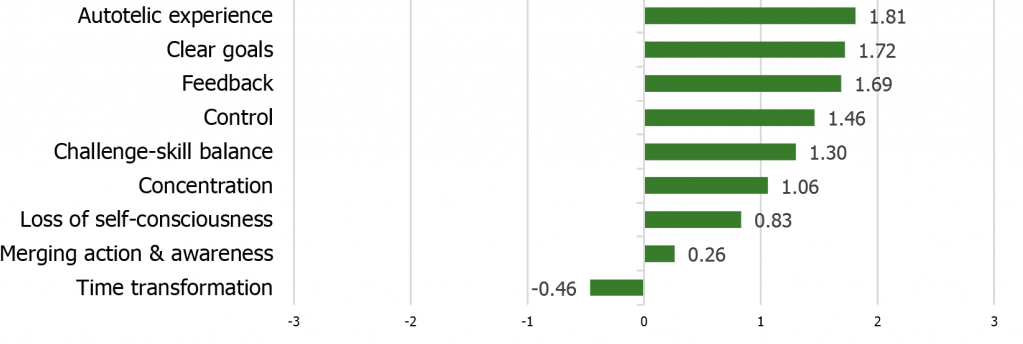
\includegraphics[width=\textwidth]{dfs2}
    \caption{Measuring flow in Gamification: Dispositional Flow Scale-2  \cite{dfs2}}
    \label{fig:dfs2}
\end{figure}
Furthermore, results also suggest that in gamifed context, the autotelic experience is highly correlated with the conditions. Hamari and Koivisto suggest that it is possible that in the Gamification context, autotelic experience truly represents a condition for reaching flow, thus implying that one can more easily reach flow if the activity is initially intrinsically motivating. 
\subsection{Motivation and Sports}

%pelletier1995toward
Vallerand (2004) states that motivation in sports matters, as it ``represents one of the most important variables in sport''. It is known to be a key element of success in sport and athletes' persistence with an exercise regiment \cite{vallerand2007intrinsic}. Intrinsic and extrinsic motivation have been particularly popular topics that allowed researchers to explain various phenomena of importance in sport and physical activity. Various studies in the domains of health, physical education, exercise and sport have explored the SDT derived hypothesis that intrinsically relative to extrinsically motivated behavior  
TODO...\\*
Armed with a clear understanding of the theory behind human motivation, this section will shed light on game elements (mechanics/dynamics), player types and the theory of flow in context of Gamification. The goal of this section is to provide a brief overview of the most relevant key elements, based on the research done on motivational theory and Gamification literature.

\subsection{Defining Gamification}
As  the  term  itself  is  relatively  new,  there  exist  numerous definitions  of  Gamification  (Zicherman \&  Cunningham 2011, Kapp 2011, Werbach \& Hunter 2012). Definition by Deterding \textit{et al.} (2011) is currently the most cited definition of Gamification in academia and is the definition that is adopted for this thesis. In their paper the authors proposed a well reasoned definition as follows:
\begin{quotation}
\textit{``Gamification is the use of game design elements in a non-game context.''}
\end{quotation}
There exist references to \textit{gamifying} online systems as early as 1980. Professor Richard Bartle from University of Essex, points out the word referred originally to ``turning something not a game into a game.''\cite{werbach2012win}%ovo je knjiga, daj stranu 
However, the first use of gamification in its current sense dates back to 2002 by Nick Pelling as part of his consultancy business, but the term did not see widespread adoption before the second half of 2010 \cite{marczewski2013gamification}. In parallel with this term, a verb \textit{to gamify} emerged. Its meaning refers to applying game mechanics to supercharge user engagement, loyalty and fun \cite{toGamify}. 
It should be noted that the definition outlined by Deterding \textit{et al.} relates to \textit{games} and not \textit{play} \cite{deterding2011game}. %Consequently, the definition distinguieshes between \textit{gamefullness} and \textit{playfullness} ... TODO. 
Even though often used interchangeably, there exists a complex relationship between these two concepts and clear distinction can be made. That is, according to the forms they take in the world, \textit{play} can be interpreted as a broader category that includes \textit{game} as a subset \cite{salen2004rules}. Play is normally assumed to be a free-form activity lacking constraints engaged in for pleasure and amusement rather than a serious or practical purpose, whereas games provide context for actions and are limited in action by fixed rules \cite{juul2011half}. In addition, Salen \& Zimmerman (2004) define game as a system where players engage in an artificial conflict which is defined by rules that limit player's behavior and define the game, that can result in a quantifiable outcome or goal \cite{salen2004rules}. %behavioral, game-playing
Games manifest themselves as integrated experiences, but they are built from many smaller pieces often called game elements \cite{werbach2012win}. They represent parts of games used as a building blocks for creating gamified applications, as well as tools and rules that define the overall context of game \cite{gamDesElem}. This means that the definition distinguishes Gamification from other systems that employ full-fledged games rather than elements of game design only. Furthermore, it does not include all game elements either, only a subcategory called game design elements that are used as seen the most suitable in current situation. %ova dve poslednje recenice odavde, izmeni 
%http://ludus.hu/en/gamification/
The final aspect of the definition is that gamification operates in non-game contexts. A non-game context refers to applications which main purpose is beyond pure entertainment; using game design elements to a context of ``other than games''. This implies that gamification can be used and successfully applied to almost anything: from business, finance, personal improvement to education, health and fitness \cite{deterding2011game}. Thus, the challenge of Gamification, is to select elements that normally operate within the game universe and apply them effectively in the real world.
%Although it is possible to also use gamification in the context  of  games  and  gamify  them,  it  can  simply  be  considered  to  be  a  part  of  designing  a  game.  This  way  specifying  gamification  to  nongame  contexts  is justified. (Deterding et al. 20
The concept of gamification is closely related to similar pre-existing concepts such as serious games, playful design and toys. Thus, the proposed definition aims at separating the concept of gamification from similar phenomena on a two-by-two matrix introduced by Deterding \textit{et al} (2011, Figure \ref{fig:mesh1}). 
\begin{figure}[h]
    \centering
    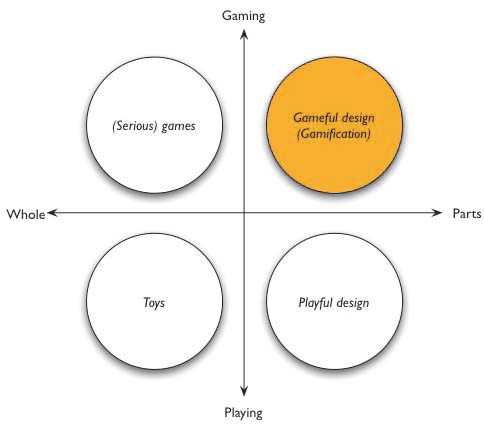
\includegraphics[width=0.75\textwidth]{gamification-btw-game-and-play}
    \caption{The matrix distinguishing the concepts related to gamification}
    \label{fig:mesh1}
\end{figure}
In figure \ref{fig:mesh1}, along one axis a distinction between gaming and playing is made, and on the other between whole game and an artifact with game elements. Gameful design or gamification, differs from playful design because the former focuses on activities that are goal oriented and structured by rules, while the latter focuses on activities that are based on improvisation and are free of form. Moreover, gamification is situated in the quadrant involving games and game elements, meaning that gamification makes use of gameful design rather than playful design and game elements rather than full-fledged games. This is different to serious games used also in non-game contexts, a group that includes full games that have been created for reasons other than pure entertainment. 
\subsection{Classification of Game elements}
% \cite{schobel2016agony}.% Sch{\"o}bel \textit{et al.} carried out a literature review to analyze the gamification elements used in various research studies.
%prezentacija o game vs play http://gamification-research.org/2012/04/defining-gamification/
%detering definise elements of game design. five leveles.Next the most common
%Next, and overview and various classification frameworks of game elements which might further enhance engagement, the potential goal of gamification is presented. 
%In a few words, the gamification process can be described as the adoption of some techniques inherited from game design into different situa-tions, other than games. In this perspective, the application of the typical game elements and the exploitation of common game design patterns are used to the aim of making some activities more appealing. In this way, users are stimulated to complete tasks by the desire of getting some rewards (Werbach & Hunter, 2012). Hence, gamification is not related to solve difficult puzzles or avoid tricks but it is the finding of effective ways to drive individuals to their goals faster. Through gamification, people feel involved in the process and are called to be proactive so that they can empower their own abilities and enhance their attitudes both online, in virtual worlds, and offline, in real world situations. Currently, gamification is used by industries to enhance the outcome of their communication campaigns and to drive the attention of people to advertising and marketing messages, in order to maximize their outcome.To conclude, gamification requires a deep understanding of what we can learn from games, so that we can design enjoyable environments and raise passion for the game we are playing  Applying gamification techniques to enhance the effectiveness of video-lessons. Available from: https://www.researchgate.net/publication/283469412_Applying_gamification_techniques_to_enhance_the_effectiveness_of_video-lessons [accessed Mar 5, 2017].
In their book \textit{Gamification by design}, Zimmerman and Cunningham (2011) argue that one should leverage aspects of game design, by focusing on it's core elements, when creating a gamified experience in order to achieve the
greatest impact for players. However, the goal of Gamification is not to build a ``full-fledged game'' but to use game elements in order to provide a gamified experience and enrich the application to engage and motivate the users \cite{werbach2012win, deterding2011game}. With respect to the use of game elements, Gamification studies classified them differently and 
there have been different attempts to create lists of those game  elements,  which  can  be applied in Gamification \cite{werbach2012win, deterding2011game, kapp2012gamification, zichermann2011gamification}. Derived from the available literature, Deterding \textit{et al.} found that game elements previously identified and presented in different research studies, fell in five distinct levels of abstraction. Table \ref{table:gameElements} presents a model for classification of game elements with five levels of abstraction, ordered from concrete to abstract. Kapp (2012), on the other hand, lists  typical  game  elements  like  goals, time, rules  conflict,  competition,  cooperation, reward  structures,  feedback,  levels,  storytelling,  curve  of  interest  and  aesthetics \cite{kapp2012gamification}.
\begin{table}[!htbp]
\centering
\caption{Taxonomy of game design elements by level of abstraction by Deterding \textit{et al.} (2011)}
\label{table:gameElements}
\begin{tabular}{lll}
\hline
\textbf{Level} & \textbf{Description} & \textbf{Example} \\ \hline
\begin{tabular}[c]{@{}l@{}}Game interface\\ design patterns\end{tabular} & \begin{tabular}[c]{@{}l@{}}Common, successful interaction\\  design components and design \\ solutions for a known problem\\  in a context, including prototypical\\  implementations\end{tabular} & \begin{tabular}[c]{@{}l@{}}Badge, leaderboard, \\ level\end{tabular} \\ \hline
\begin{tabular}[c]{@{}l@{}}Game design\\ patterns and\\ mechanics\end{tabular} & \begin{tabular}[c]{@{}l@{}}Commonly reoccurring parts of \\ the design of a game that\\  concern gameplay\end{tabular} & \begin{tabular}[c]{@{}l@{}}Time constraint, \\ limited resources, turns\end{tabular} \\ \hline
\begin{tabular}[c]{@{}l@{}}Game design\\ principles and\\ heuristics\end{tabular} & \begin{tabular}[c]{@{}l@{}}Evaluative guidelines to approach a\\  design problem or analyze a given\\ design solution\end{tabular} & \begin{tabular}[c]{@{}l@{}}Enduring play,\\ clear goals, \\ variety of game styles\end{tabular} \\ \hline
Game models & \begin{tabular}[c]{@{}l@{}}Conceptual models of the components of\\  games or game experience\end{tabular} & \begin{tabular}[c]{@{}l@{}}
MDA; challenge, \\ fantasy, curiosity;\\ game design atoms; \\ Core Elements of the \\ Gaming Experience \end{tabular} \\ \hline
\begin{tabular}[c]{@{}l@{}}Game design\\ methods\end{tabular} & \begin{tabular}[c]{@{}l@{}}Game design-specific\\  practices and processes\end{tabular} & \begin{tabular}[c]{@{}l@{}}Playtesting,\\ playcentric design, \\ value conscious\\ game design\end{tabular} \\ \hline
\end{tabular}
\end{table}\\*
Zichermann \& Cunningham (2011) take a different approach and base their description of game elements on the MDA framework, which is categorized as a \textit{game model} in the framework proposed by Deterding \textit{et al.} (2011). It is one of the most frequently used frameworks of game design and stands for \textit{Mechanics}, \textit{Dynamics} and \textit{Aesthetics} \cite{hunicke2004mda}. 
Introduced by Robin Hunicke, Mark LeBlanc and Robert Zubek, the MDA framework formalizes games consumption by breaking them into their distinct elements: rules, system and "fun". These elements translate into the following design counterparts which constitute the MDA` framework: Mechanics, Dynamics and Aesthetics \cite{hunicke2004mda}. Mechanics are the functioning components that make up the game. They represent the specific elements of the game and the different behaviors and control mechanism that are given to the player within the game's context. Dynamics, on the other side, represents player’s interactions with the mechanics. They specify how the player reacts to the mechanics of the system, both individually and with other players. Lastly, the aesthetics of the system are the emotional reponses of the users who interact with the game system \cite{zichermann2011gamification}. This framework has been very influential in helping designers and theorists conceptualize different aspects of games and how to create them. In their book \textit{For the Win. How Game thinking can revolutionize your business} Werbach and Hunter (2012) introduce three categories of game elements that are relevant to Gamification, which are: \textit{Dynamics}, \textit{Mechanics}, and \textit{Components}. These terms are similar to the ones used in the MDA framework, although LeBlanc \textit{et al} use these terms in different ways. Werbach and Hunter, organized Gamification elements in decreasing order of abstraction where each mechanic is tied to one or more dynamics, and each component is tied to one or more higher-level elements (see Figure \ref{fig:mdc}).
\begin{figure}[h]
    \centering
    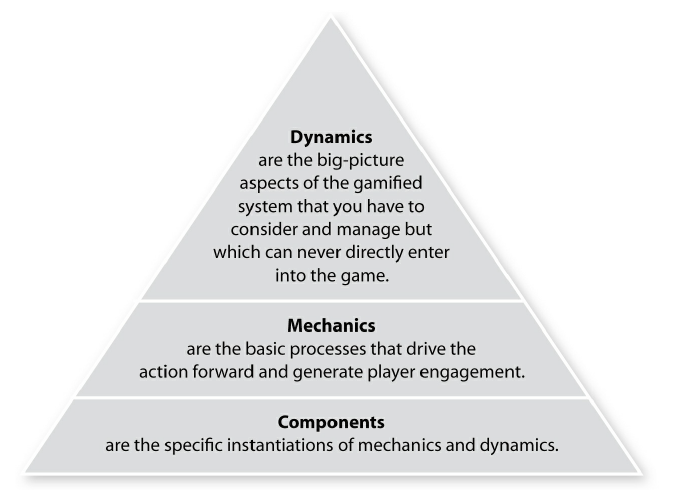
\includegraphics[width=0.75\textwidth]{mdc}
    \caption{The Pyramid of Game Elements from Werbach \& Hunter (2012, p. 82)}
    \label{fig:mdc}
\end{figure}
In the next section different mechanics, dynamics and components are listed and described according to their relevance and applicability to our context.
\subsubsection{Dynamics}
At the highest level of abstraction are game dynamics and serve as the core,  underlying framework for the Gamification to take place. Furthermore, they represent the implicit structure that guide the game, set  up  the  rules and constraints and  define the overall purpose, aim and goal of the game \cite{werbach2012win, WerbachCoursera}. 
According to Werbach and Hunter, the most important game dynamics are \cite{werbach2012win}:
\begin{itemize}
\item \textbf{Constraints}(limitations or forced trade-offs).  Every game has some constraints, because games create meaningful choices and interesting problems by limiting people's freedom. So the notion of what constraints get put on users is an important dynamic that any game designer needs to think about. 

\item \textbf{Emotions}. Games can produce various emotions, from joy and sadness to everything in between. However, Werbach argues that the emotional palette of gamification is typically somewhat more limited \cite{WerbachCoursera}. The reason for this is because Gamification deals with real world, non-game context, such as marketing, or exercise context. In contexts like those, getting someone, for instance, really upset, will probable not be beneficial and valued. But there still are a variety of emotional levers that can be pulled, that can make the experience more rich, and certainly the joy, the, the sense of accomplishment, the emotional reinforcement that pushes people to play more, is important in most examples of gamification. 
\item Narrative (a consistent, ongoing storyline) Narrative: the structure that pulls together the pieces of the game, or the gamified system into some coherent feeling whole. The narrative can be explicit, the storyline in a game, or it can be implicit. And gamification doesn't necessarily have the richness of the aesthetic experiential aspect of games to put the work in creating a narrative. It has to rely upon things like consistent graphical experiences, creating a sense of flow and alluding to certain kinds of practices or certain kinds of story ideas that may be in players' heads using those, again, to tie together the individual pieces. If there's no sense of narrative, then the risk is that the gamified system will just be a bunch of abstract stuff. You get these badges. You get these points, but they're totally divorced from any sense of coherence and relation to the player's life and that tends to limit the effectiveness of gamification.
\item Progression (the player's growth and development)
\item Relationships (social interactions generating feelings of camaraderie, status, altruism, and so on)
\end{itemize}
\subsubsection{Mechanics}
Kevin Werbach describes game mechanics as ``the processes that drive actions forward''. He subsequently compared mechanics to ``verbs'' which help people to play games (see Fig. 2). In their academic article, Robert Hunicket et al. defined game mechanics as “the particular components of the game, at the level of data representation and algorithms”.

Mechanics are the basic processes that drive the action forward and generate player engagement. We
can identify ten important game mechanics:

\begin{itemize}
\item Challenges (puzzles or other tasks that require effort to solve)
\item Chance (elements of randomness)
\item Competition (one player or group wins, and the other loses . . . )
\item Cooperation (players must work together to achieve a shared goal)
\item Feedback (information about how the player is doing)
\item Resource Acquisition (obtaining useful or collectible items)
\item Rewards (benefits for some action or achievement)
\item Transactions (trading between players, directly or through intermediaries)
\item Turns (sequential participation by alternating players)
\item Win States (objectives that makes one player or group the winner—draw and loss states are
related concepts)
\end{itemize}
\subsubsection{Components}
Components make up the largest fraction of game elements. They can be viewed as more-specific forms that mechanics or dynamics can take. These elements are less abstract than the categories described previously and lead to tools that can be used in order to begin incorporating Gamification in the environment of interest. There many game elements that can be successfully used in gamified environments. However, some are more common than others, and some are more influential in shaping typical examples of gamification. Werbach and Hunter examined over 100 implementations of Gamification and claim that three elements always appear: \textit{points, badges}, and \textit{leaderboards}. They further point out how these elements are so common within Gamification that ``they are often described as though they are Gamification'', even though they are not \cite{werbach2012win}.  Hamari \textit{et al.} (2014), in their comprehensive survey of peer-reviewed empirical studies on gamification, also found that these three elements ``were clearly the most commonly found variants" in the large variety of elements tested \cite{hamari2014does}. The same elements were listed and described by Zichermann (2011), alongside \textit{levels}, \textit{challenges/quests}, \textit{onboarding}, and \textit{engagement loops} \cite{zichermann2011gamification}. In the next section, these three elements, commonly represented by the acronym \textit{PBL}, will be discussed.

\begin{enumerate}
\item \textbf{Points}\\*
Points represent a running numerical value which is given for any single action or combination of actions. In Gamification, they are mostly used to encourage people to do things by collecting them. The main assumption is that players will work harder in exchange for points. This is a very simple approach that occasionally works in motivateing those payer types who like collecting things or who like competing against each other. According to Zichermann and Cunningham (2011) points are ``an absolute requirement for all gamified systems'' and can serve a wide range of purposes, from obvious to barely visible ones. One of the most obvious usage of points and points systems is to for keeping a score. This way, points also provide a way of determining how well someone is doing in the game. So points can either show the relative position of players or they can actually define winning \cite{WerbachCoursera}. Werbach argues that points can also create a connection between progression in the game and extrinsic rewards since gamified systems offer some real-world prizes for reaching certain levels or number or virtual points. Another purpose for points is to provide feedback of the action. Explicit and frequent feedback represent a key element in most good game design, and points provide feedback quickly and easily and, by doing so, they show, in real time, how one is doing in the game. Finally, points provide data for the game designer since the points that users earn can easily be tracked and stored which allows the designer to analyze important metrics about the system. Zichermann and Cunningham (2011) distinguish five categories of point systems. According to the authors, points  can  be  divided  into  different categories  according  to  their  function. That is, one can differentiate among the following point systems: 
\begin{itemize}
\item Experience points,
\item Redeemable points,
\item Reputation points, 
\item Skill points, and
\item Karma  points
\end{itemize}
Each of the mentioned type of point system can have significantly different tasks in the gamified context. Even though, they can be a powerful motivator, Werbach and Hunter state that points are, in fact, very limited because of their uniform, abstract, interchangeable nature. That is, a point is only a point and nothing more. This is one of the reasons why badges are often found in conjunction with points systems.
\item Badges
A badge is a visual representation of some achievement
within the gamified process. (The terms “badges” and “achievements” are often used synonymously in
gamification.) Some badges simply demarcate a certain level of points.

Researchers Judd Antin and Elizabeth Churchill suggest that a well-designed badge system has five
motivational characteristics:
1. Badges can provide a goal for users to strive toward, which has been shown to have positive
effects on motivation.
2. Badges provide guidance as to what is possible within the system and generate a kind of
shorthand of what the system is supposed to do. This is an important feature for “onboarding,” or
getting the user engaged with the system.
3. Badges are a signal of what a user cares about and what he or she has performed. They are a
kind of visual marker of a user’s reputation, and users will often acquire badges to try to show
others what they are capable of.
4. Badges operate as virtual status symbols and affirmations of the personal journey of the user
through the gamification system.
5. Badges function as tribal markers. A user who has some of the same badges as other users will
feel a sense of identity with that group, and a clever gamification design can connect the badges
with a system of group identification.
One of the most important attributes of badges is their flexibility. Many different kinds of badges can
be awarded for many different kinds of activity, and the range of badges is limited only by the
imagination of the gamification designer and the needs of the business. This allows the gamified
service to engage a more diverse group of users and to appeal to their interests in ways that a single
points system cannot.
\item Leaderboards
\end{enumerate}


The fifteen important game
components are:

\begin{itemize}
\item Achievements (defined objectives)
\item Avatars (visual representations of a player's character)
\item Badges (visual representations of achievements)
\item Boss Fights (especially hard challenges at the culmination of a level)
\item Collections (sets of items or badges to accumulate)
\item Combat (a defined battle, typically short-lived)
\item Content Unlocking (aspects available only when players reach objectives)
\item Gifting (opportunities to share resources with others)
\item Leaderboards (visual displays of player progression and achievement)
\item Levels (defined steps in player progression)
\item Points (numerical representations of game progression)
\item Quests (predefined challenges with objectives and rewards)
\item Social Graphs (representation of players' social network within the game)
\item Teams (defined groups of players working together for a common goal)
\item Virtual Goods (game assets with perceived or real-money value)
\end{itemize}

%just for health and fitness gamification
%First  the  elements  most related   to   motivation   are   presented   and   then   the   most   popular elements   in gamification  literature  are  presented.  Although  all  game  elements  can be  used  in gamification they might not all be equally relevant. Some are more potent and useful than others. As it is also a goal of this paper to examine which elements are the most  relevant,  based  on  the  research  done  on  motivational  theory  and  gamification literature a distinction is made.
%In theory, any context, task or process can be gamified \cite{muntean2011raising}. %skini i procitaj Muntean!! 

\subsection{User Types}

\begin{figure}[h]
    \centering
    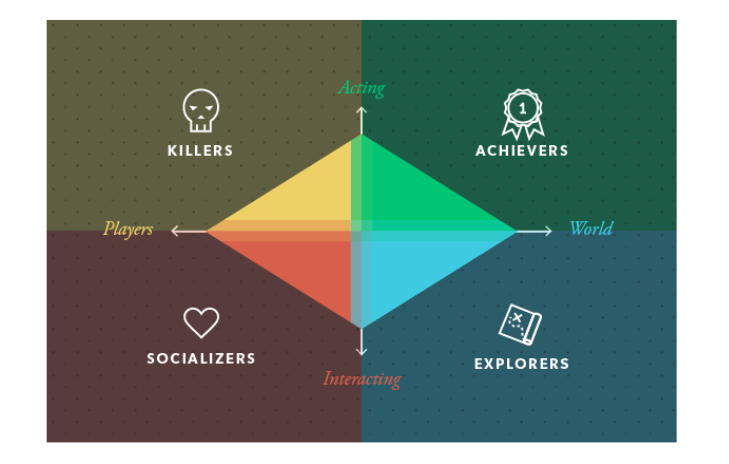
\includegraphics[width=0.75\textwidth]{userTypes}
    \caption{User types}
    \label{fig:userTypes}
\end{figure}
%\subsection{Objectives}
%\subsection{Principles}
%\subsection{The impact of Gamification}
%\subsubsection{Gamification in sports - Effects and Objectives}
%The main goal of gamification is to engage the users Gamification’s main goal is to rise the engagement of users by using game-like techniques such asscoreboards and personalized fast feedback (Flatla et al, 2011) making people feel more ownership and purpose when engaging with tasks (Pavlus, 2010).\cite{burke2016gamify}
%\subsection{Gamification critiques}
\subsection{Gamification of Health and Fitness}
Gamification in Health and Fitness has rapidly emerged over the past decade as a tool to promote health and wellness. It is a broad term referring to the use of game thinking and game mechanics in a non-game context to engage users and solve problems. %The concept is used to incentivise users to achieve their goals and increase user engagement. The best examples of gamification are in the Health and Fitness industry, where games encourage exercise by turning physical activity into a game and by delivering health interventions for bad habits cessation, like smoking, overeating or poor hydration, and medication adherence. Application of mobile and wearable devices have proven to be effective platforms for health and fitness games due to its wide adaptation, ease of use and continuous proximity to the users and patients. Since gamification can be applied to almost any business model, serious or not, for this thesis, we restrict our concern of gamification to the solving of serious issues. In particular, we are focused on gamification of education and behavior change related to the serious world issue of childhood obesity
